\section{Select data source/Assign columns}
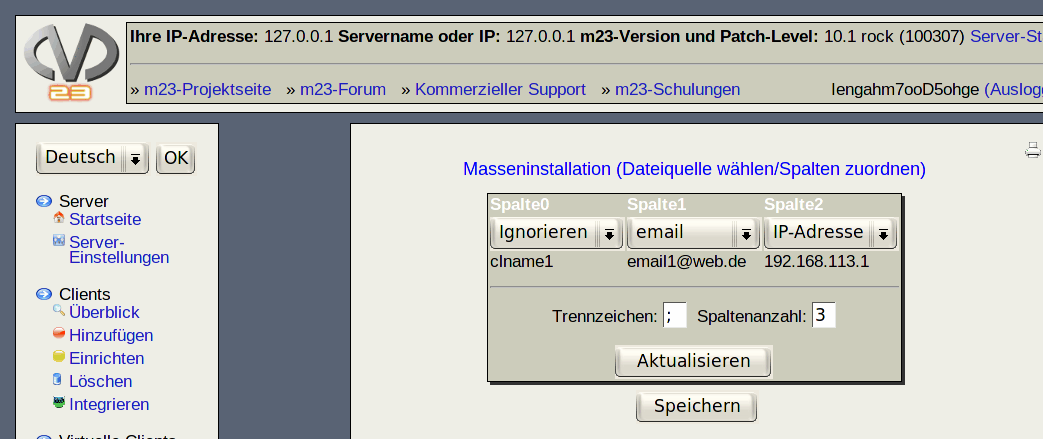
\includegraphics[scale=0.33]{/mdk/doc/manual/screenshots/en/mi_step2.png} \\
This dialog is divided into two steps:\\
\begin{itemize}
\item Select and upload a database file\\
\item Assign the fields to the client options\\
\end{itemize}
\subsection{Select and upload a database file}
Select a file with the diealog and click on \textit{"Upload"}.\\
A special data format is needed to make the value recognition possible for m23. The values for a single client are specified in every line. The client options are separated by a separator character (here ";")::\\
\begin{verbatim}
option1;option2;option3;...
\end{verbatim}
You can use other combinations of a maximum of 4 characters. The order of the options has to be the same in all lines.\\
\subsection{Hint}
All in the file stored values have to be valid and there are an additional requirements for special options:\\
\begin{itemize}
\item \textbf{Store login information local on the client.}: Set it to "yes" if you want to activate this option. All other values disable it.\\
\item \textbf{LDAP}: Here three different values are possible:\\
\begin{itemize}
\item "none": Don't user LDAP\\
\item "read": Read login information from selected LDAP server.\\
\item "write": Store login information on the selected LDAP server.\\
\end{itemize}
\end{itemize}
\subsection{Assign the fields to the client options}
You can assign the fields to the option names after uploading a file.\\
\subsection{Step by step}
\begin{enumerate}
\item Enter the separator character in the separator field and adjust the column amount if needed.\\
\item Click on \textit{"Refresh"}. The first line of the database file is now separated and shown in the client option fields.\\
\item Assign the separated parts from the database file to the client options by selecting the client option names from the selection list.\\
\item End the dialog with a click on \textit{"Save"}.\\
\end{enumerate}
